\section{Zielsetzung}
\label{sec:Zielsetzung}
Ziel des Versuches ist es, die mittlere Lebensdauer von kosmischen Myonen mittels eines Szintillationsdetektors zu bestimmen. 

\section{Theorie}
\label{sec:Theorie}
\subsection{Eigenschaften und Entstehung kosmischer Myonen}
Myonen, $\mu$, sind Elementarteilchen des Standardmodells der Teilchenphysik. Sie gehören zu der Familie der Leptonen und werden zusammen mit ihrem zugehörigen Neutrino $\nu_\mu$ in der zweiten Generation eingeordnet \ref{fig:std}.
\begin{figure}[H]
    \centering
    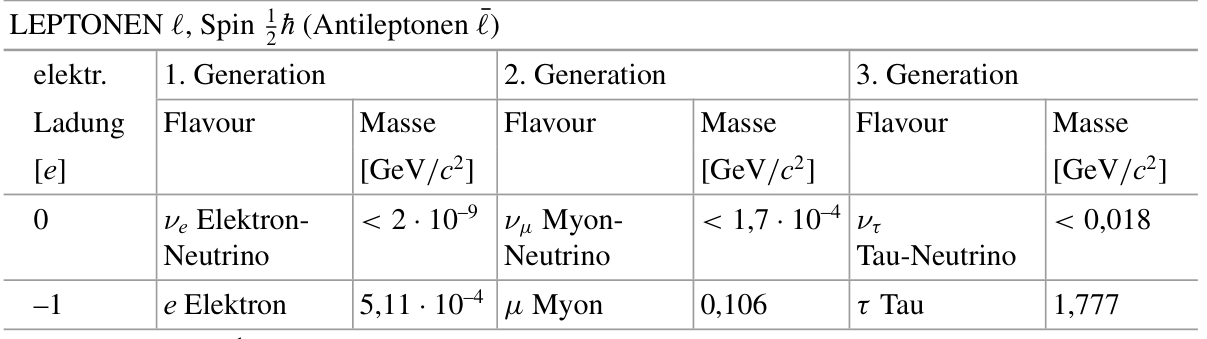
\includegraphics[width=\linewidth]{data/leptonen_std.png}
    \captionof{figure}{Die drei Leptonengenerationen des Standardmodells \cite{astro}}
    \label{fig:std}
\end{figure}
\noindent
Myonen haben Spin $\frac{1}{2}$ und sind daher Fermionen. Sie haben eine negative Ladung von $q = \SI{-1}{e}$ und wiegen mit $m_\mu \approx \SI{106}{MeV}$ ca. $200$ mal so viel wie ein Elektron mit $m_e \approx \SI{0.511}{keV}$. Die in diesem Versuch zu bestimmende mittlere Lebensdauer der Myonen beträgt $\tau_{\mu} = \SI{2.2}{\micro\second}$ \cite{pdg}, diese Zerfallen zu ca. 100\% \cite{pdg} über ein $W^{-}$ Boson in ein Elektron und zwei Neutrinos, nach 
\begin{equation}
    \mu^- \rightarrow e^- + \bar{\nu}_e + \nu_\mu
\end{equation}
Kosmische Myonen entstehen in einer höhe von ca. $\SI{20}{km}$ in sogenannten Luftschauern. Diese finden statt, wenn ein hochenergetisches Teilchen aus dem kosmos auf die Erdatmosphäre trifft und dort mit den Teilchen dieser wechselwirkt.
Bei nicht zu hohen Energien sind Protonen die häufigsten Primärteilchen. Diese Treffen auf die Atmosphäre und zerfallen bei der Wechselwirkung mit den Atomen und Molekülen der Erdatmosphäre in Kaonen und Pionen. Kaonen und Pionen zerfallen weiter in Myonen, wie hier Beispielhaft für $K^-$ und $\pi^-$ nach
\begin{equation}
    \begin{aligned}
        K^- &\rightarrow \mu^- &+ \bar{\nu}_\mu \\
        \pi^- &\rightarrow \mu^- &+ \bar{\nu}_\mu
    \end{aligned}
\end{equation}
welche als häufigstes Teilchen auf Meereshöhe gemessen werden.
\begin{figure}[H]
 \centering
 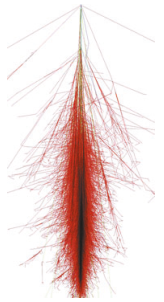
\includegraphics[width=0.2\linewidth]{data/Luftschauer.png}
 \captionof{figure}{Simulation eines Luftschauers, ausgelöst durch ein kosmisches Proton bei $E_p = \SI{1}{TeV}$ \cite{astro}}
 \label{fig:luftschauer}
\end{figure}
\noindent
Grund für das erreichen des Bodens der Myonen sind relativistische Effekte. Ein Myon mit einer Energie von $E_{\mu} = \SI{10}{GeV}$ fliegt nach 
\begin{equation}
    \label{eqn:t1}
    v_\mu = \frac{\frac{p_\mu}{m_\mu}}{\sqrt{1 + \left( \frac{p_\mu}{m_\mu} \right)^{2}}}
\end{equation}
mit einer Geschwindigkeit von ca. $v_{\mu} \approx 0.9999 \cdot \symup{c}$, wobei sich $p_\mu$ durch 
\begin{equation}
    p_\mu = \sqrt{E_\mu^2 - m_\mu^2}
\end{equation}
berechnen lässt.
Ein Teilchen mit dieser Geschwindigkeit hat somit einen Gamma Faktor von $\gamma_\mu \approx 90$. Bei einer mittleren Lebensdauer von $\tau_{\mu} = \SI{2.2}{\micro\second}$ \cite{pdg} berechnet sich die aus dem ruhendem System auf der Erdoberfläche zurückgelegte mittlere Strecke des Myons dann nach 
\begin{equation}
    \label{eqn:t2}
    s = v_{\mu} \cdot \tau_{\mu} \cdot \gamma_{\mu}
\end{equation}
auf $s \approx \SI{60000}{m}$. Bei einer klassischen Rechnung beträgt dieser Wert $s_{\symup{klassisch}} \approx \SI{650}{m}$.
\subsection{Zerfallsgesetz und mittlere Lebensdauer}
Die mittlere Lebensdauer eines Myons lässt sich aus dem Zerfallsgesetz 
\begin{equation}
    \label{eqn:t3}
    \symup{d}N = - \lambda N \symup{d}t
\end{equation}
herleiten. Dieses besagt, dass die Änderung der Anzahl an Teilchen $N$ um $\symup{d}N$ antiproportional ist zu einer Konstante $\lambda$ mal der Anzahl der Teilchen $N$ im Zeitintervall $\symup{d}t$. Aus dieser Differentialgleichung folgt, dass die Menge $N$ der nach der Zeit $t$ noch vorhandenen Teilchen der Funktion
\begin{equation}
    \label{eqn:t4}
    N\left(t\right) = N_0 \cdot \symup{exp} \left( -\lambda t \right)
\end{equation}
folgt. Dabei ist $N_0$ die Anzahl der Teilchen bei $t = 0$. Für den Fall, dass $N_0 = 1$ ist, also dass wir ein Teilchen betrachten, betrachten wir eine Verteilungsfunktion der Form 
\begin{equation}
    \label{eqn:t5}
    P\left(t\right) = \symup{exp} \left( -\lambda t \right) .
\end{equation}
Gleichung \ref{eqn:t5} gibt dabei die Wahrscheinlichkeit an, dass das betrachtete Teilchen nach der Zeit t noch nicht Zerfallen ist. Die Funktion $P\left(t\right)$ impliziert so die existenz einer Wahrscheinlichkeitsdichte der Form
\begin{equation}
    \label{eqn:t6}
    p\left(t\right) = \lambda \cdot \symup{exp} \left( -\lambda t \right) 
\end{equation}
wobei der Zusammenhang $\symup{d}P\left(t\right) = p \left(t\right) \symup{d}t$ gilt.
Die Wahrscheinlichkeitsdichte aus Gleichung \ref{eqn:t6} bedingt den Erwartungswert
\begin{equation}
    \label{eqn:t7}
    \langle t \rangle  = \int_0^{\infty} t \cdot p\left(t\right) \symup{d}t = \frac{1}{\lambda}
\end{equation}
welcher als mittlere Lebensdauer $\tau$ identifiziert wird. Es gilt daher 
\begin{equation}
    \label{eqn:t8}
    \tau = \frac{1}{\lambda}
\end{equation}
\newpage
\subsection{Messprozess der kosmischen Myonen}
Für die Detektion der Myonen wird in diesem Versuch ein Szintillationsdetektor verwendet. Szintillatoren absorbieren Ionisierende Strahlung wodurch in dem Material Photonen ausgelöst werden. Diese entstehen Entweder durch Ionisation des Szintillatormaterials und anschließender Rekombination, oder 
durch eine Anregung der Szintillatormoleküle bei deren Abregung ein Photon abgestrahlt wird. Szintillatoren werden allgemein als organische und anorganische Szintillatoren klassifiziert. Organische Szintillatoren sind gut geeignet um Hochfrequente Messungen zu Tätigen, da die Abstrahlung der Photonen schneller stattfindet als bei anorganischen Szintillatoren. Anorganische Kristalline Szintillatoren haben gegenüber organischen Szintillatoren den Vorteil, dass diese Aufgrund Ihrer Kristallstruktur und der Resultierenden Bandstruktur feste Übergangsenergien besitzen. Aufgrund des Spektrums der Szintillator Photonen sind so also auch Energiemessungen
möglich. 

\begin{figure}[H]
    \centering
    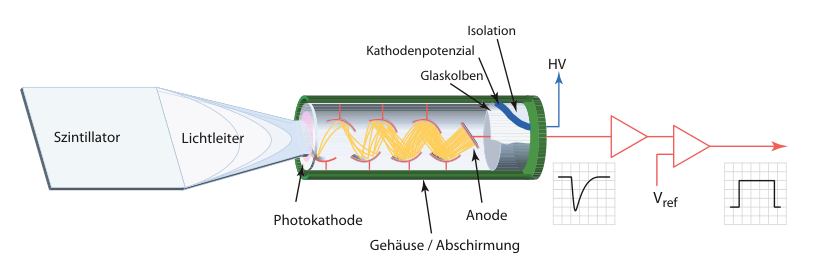
\includegraphics[width=0.8\linewidth]{data/photomult.png}
    \captionof{figure}{Schematischer Aufbau eines Photomultipliers \cite{szinti}}
    \label{fig:phot}
\end{figure}
\noindent
In \autoref{fig:phot} ist schematisch der Aufbau eines Photomultipliers zu sehen. Diese Wandeln ein Lichtsignal in ein elektrisches Signal um, welches dann weiter verarbeitet werden kann. Dies geschieht indem Einfallende Photonen aus dem Szintillator über einen Lichtleiter auf eine Photokathode gelenkt werden. In dieser Photokathode findet der
Photoeffekt statt, wodurch ein Elektron aus dem Kathodenmaterial gelöst wird. Dieses wird Aufgrund einer angelegten Hochspannung im Bereich $U_{\text{PM}} \approx \SI{2}{kV}$
\newpage


\section{Versuchsaufbau}
In \autoref{fig:aufb} ist schematisch der in diesem Versuch verwendete Aufbau zu sehen.
\begin{figure}[H]
    \centering
    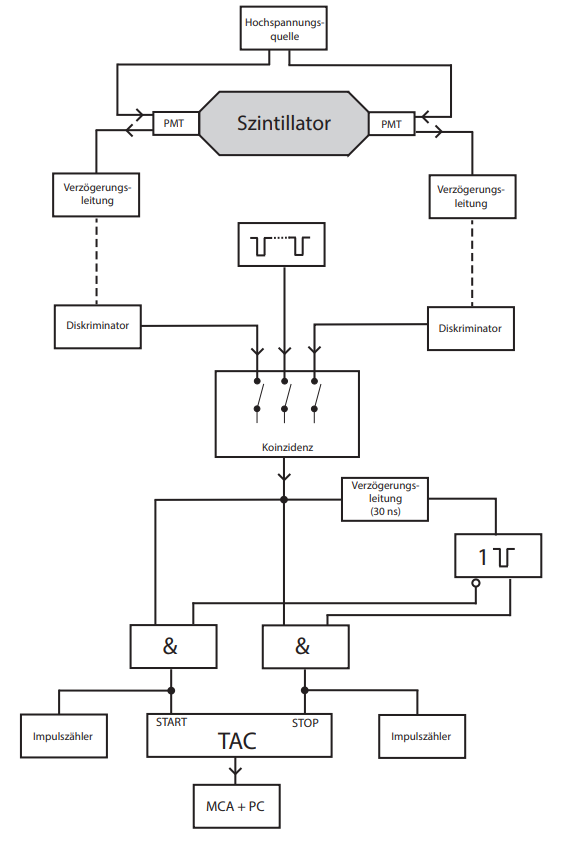
\includegraphics[width=0.5\linewidth]{data/aufbau_schem.png}
    \captionof{figure}{Schematischer Versuchsaufbau \cite{V01}}
    \label{fig:aufb}
\end{figure}
\noindent
Dieser besteht aus einem Szintillator, an welchen zwei gegenüberliegende Photomultiplier angeschlossen sind. Diese werden über eine Hochspannungsquelle betrieben und geben ein 
elektrisches Signal über jeweils eine variable Verzögerungsleitung in jeweils einen Diskriminator weiter. An den Diskriminatoren lässt sich die Ausgegebene Pulsbreite und die Akzeptanzschwelle des eingehenden Signals einstellen.
Die vom Diskriminator verarbeiteten Signale laufen in einer Koinzidenzschaltung zusammen, in welcher diese Akzeptiert werden, wenn diese "Gleichzeitig genug" eintreffen. Das Signal aus der Koinzidenzschaltung wird dreifach geteilt, wobei wie in \autoref{fig:aufb} zu sehen zwei der Signale in jeweils 
ein Und-Gatter gehen und das dritte über eine $\SI{30}{ns}$ Verzögerungsleitung in ein Monoflop. An dem Monoflop lässt sich ein Timer Einstellen, welcher die Suchzeit nach einem Zerfallssignal im Szintillator vorgibt. Das Monoflop Schaltet so nach ablauf der Suchzeit wieder das erste Und-Gatter frei welches in dem folgenden TAC ($\textbf{T}$ime $\textbf{A}$mplitude $\textbf{C}$onverter)
die Start Signale auslöst. Trifft ein Signal aus der Koinzidenzschaltung während der Suchzeit ein wird das zweite Und-Gatter ausgelöst, welches im TAC ein Stoppsignal auslöst. Das vom TAC gemessene Zeitintervall wird in eine Amplitude umgewandelt und an einen MCA ($\textbf{M}$ulti $\textbf{C}$annel $\textbf{A}$nalyser) weiter gegeben. Dieser Ordnet Die Signalamplituden gebinnten Channeln zu, sodass am PC ein Histogramm gemessen werden kann.
Zusätzlich messen zwei Impulszähler die Anzahl an Start und Stop Signalen, wobei nur jene Signale bei denen ein Stop im TAC ausgelöst wurde, auch als Datenpunkte im Histogramm zu sehen sind.
\newpage
